\subsection{Ecore Editors}

This section describes some of the existing editors for \gls{Ecore} models.
Most of them are provided in the \gls{Eclipse}.
They can be used to draw inspiration for new \gls{cloud} editors, and suggest functionalities and requirements that are needed.

\subsubsection{Sample Reflective Ecore Model Editor} %Default EMF Genmodel editor
A master-detail tree editor in \gls{Eclipse}.
It uses the \emph{reflective \acrshort{API}} of \gls{Ecore} to convert models into trees.
The source code lives in the \href{https://git.eclipse.org/c/emf/org.eclipse.emf.git/tree/plugins/org.eclipse.emf.ecore.editor/src/org/eclipse/emf/ecore/presentation/EcoreEditor.java}{org.eclipse.emf.ecore.editor} package.

A screenshot of the editor can be seen in \cref{fig:sample-reflective-ecore-model}.
It supports both models (\cref{sfig:sample-reflective-ecore-model-screenshot}) and model instances (\cref{sfig:sample-reflective-ecore-model-instance-screenshot}).

A relevant piece of the source code is the \texttt{ReflectiveItemProvider}\footnote{\href{https://git.eclipse.org/c/emf/org.eclipse.emf.git/tree/plugins/org.eclipse.emf.edit/src/org/eclipse/emf/edit/provider/ReflectiveItemProvider.java}{https://git.eclipse.org/c/emf/org.eclipse.emf.git/tree/plugins/org.eclipse.emf.edit/src/org/eclipse/emf/edit/provider/ReflectiveItemProvider.java}} from \texttt{org.eclipse.emf.edit}.
This code converts the model instances to text labels (\href{https://git.eclipse.org/c/emf/org.eclipse.emf.git/tree/plugins/org.eclipse.emf.edit/src/org/eclipse/emf/edit/provider/ReflectiveItemProvider.java#n390}{line 390}) and provides their icons (\href{https://git.eclipse.org/c/emf/org.eclipse.emf.git/tree/plugins/org.eclipse.emf.edit/src/org/eclipse/emf/edit/provider/ReflectiveItemProvider.java#n380}{line 380}), for display in a tree.
% https://git.eclipse.org/c/emf/org.eclipse.emf.git/tree/plugins/org.eclipse.emf.edit/model/Tree.ecore

\begin{figure}
    \centering
    \begin{subfigure}[b]{.45\textwidth}
        \centering
        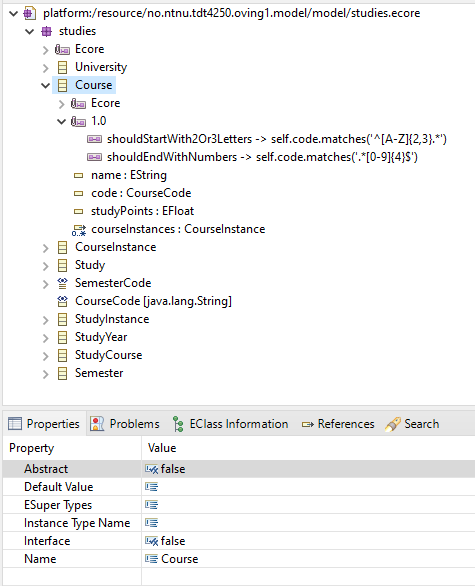
\includegraphics[width=\textwidth]{figures/ecore-sample-reflective-ecore-model-editor}
        \caption{A model opened in the editor.}
        \label{sfig:sample-reflective-ecore-model-screenshot}
    \end{subfigure}
    \hfill
    \begin{subfigure}[b]{.45\textwidth}
        \centering
        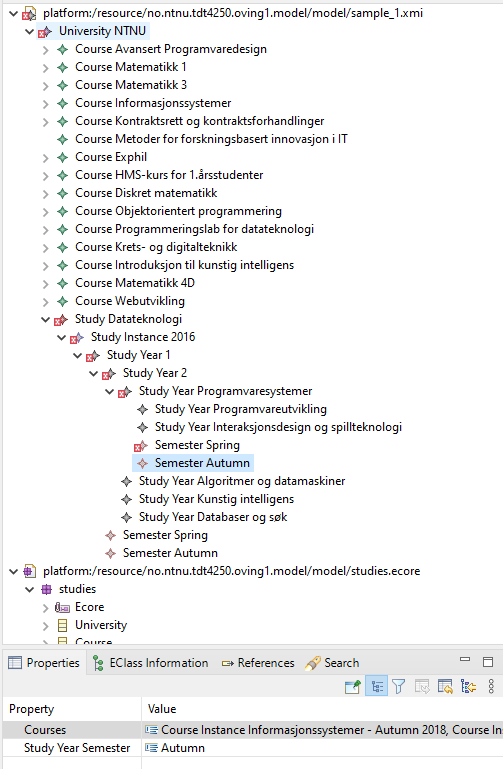
\includegraphics[width=\textwidth]{figures/ecore-sample-reflective-ecore-model-editor-instance.png}
        \caption{A \emph{dynamic instance} (\gls{XMI}) opened in the editor.}
        \label{sfig:sample-reflective-ecore-model-instance-screenshot}
    \end{subfigure}
    \caption{Screenshots of the Sample Reflective Ecore Model Editor in \gls{Eclipse}.}\label{fig:sample-reflective-ecore-model}
\end{figure}

\subsubsection{EMF Forms Ecore Editor} % EMF Forms based

\subsubsection{Ecore Tools} % Sirius based
The \emph{Ecore Tools} editor is based on Sirius (see \cref{sec:sirius}).
It displays diagrams as \gls{UML} Class Diagrams.

\subsubsection{ecore-glsp} %Theia
